\label{sota}
\minitoc
\section{Modalités des circulations des savoirs}
De nombreux$\cdot$ses chercheur$\cdot$se$\cdot$s$\cdot$x partagent le point de vue selon lequel la notion de circulation des savoirs constitue un champ de recherche vaste, ainsi qu'un nouveau paradigme de la connaissance depuis le début du XXI\ieme{} siècle et l'avènement du Web \textsc{2.0} (\citealp{landais2014frederic,quet2014frederic}). Cette phase de l'évolution du Web se caractérisait notamment par la transformation majeure de l'Internet en vue du développement des réseaux sociaux, des blogs et des sites participatifs, tout en permettant aux utilisateur$\cdot$trice$\cdot$s$\cdot$x de créer, partager et interagir avec du contenu Web. Nous traversons actuellement l'ère du Web \textsc{3.0}, né dans les années 2010 et appelé également \og{}Web sémantique\fg{}, qui permet de lier et structurer l'information afin d'en extraire la connaissance (\citeauthor{andrade2013sociologie} \citeyear{andrade2013sociologie}, p.~107). Néanmoins, en parlant de la circulation des savoirs, \citeauthor{landais2014frederic} (\citeyear{landais2014frederic}, p.~331) remarque que ce phénomène connaît une croissance importante grâce aux outils de la numérisation de la production scientifique et de l'édition numérique des ouvrages.
%les savoirs sont amenés à circuler, à voyager, à se propager, mais aussi à communiquer plus rapidement ce qui ouvre de nombreuses pistes de recherche, aussi bien théoriques qu'appliquées, orientées vers l'exploration de la nature de ces circulations. 

Le terme en question reste toutefois assez complexe en raison de visions différentes sur la façon de le définir. Afin d'éclairer cette problématique, \citeauthor{quet2014frederic} (\citeyear{quet2014frederic}, pp.~221--222) souligne trois aspects suivants :
\begin{enumerate}
    \item \textbf{Éléments de la circulation}. Qu'est-ce qui circule ? 
    \begin{itemize}
        \item individus (savants, techniciens, traducteurs, etc.) ;
        \item objets matériels (instruments scientifiques, ouvrages etc.) :
        \item constructions symboliques (théories, concepts etc.).
    \end{itemize}  
    \item \textbf{Conceptions de la circulation et méthodes de son analyse} ;
    \begin{itemize}
        \item définition de la circulation comme \og{}traduction\fg{}, \og{}diffusion\fg{}, \og{}accès\fg{} ou \og{}succès\fg{} ;
        \item critères méthodologiques possibles pour étudier la circulation p. ex. d'une théorie : 
        \begin{itemize}
            \item circulations géographiques des principaux concepteurs qu'on lui reconnaît ;
            \item circulations et lectures des textes produits par leurs concepteurs ;
            \item usages et applications analogiques qui en sont faits dans d'autres domaines.
        \end{itemize} 
        \item enjeux d'articulation de ces différents niveaux d'observation du point de vue méthodologique et de celui de la production du texte de recherche, dans le cas des croisements de ces niveaux.
    \end{itemize}
    \item \textbf{Conceptions analytiques et normatives des savoirs}
    \begin{itemize}
        \item affaiblissement des catégories des \og{}savoirs profanes\fg{} et \og{}savoirs scientifiques\fg{}, ainsi que de l'opposition entre eux ;
        \item revalorisation des savoirs implicites et de la dimension pratique des connaissances ;
        \item glorification de la circulation comme porteuse de valeurs \textit{a priori} positives : confrontation à l'autre, hybridation, production de nouveauté, etc.
    \end{itemize}
\end{enumerate}

Dans le cadre de l'analyse de l'impact scientifique de Charcot, nous étudions \textit{in fine} la circulation de ses théories et des concepts médicaux dont il était inventeur (p. ex. \textit{SLA}) et transmetteur (p. ex. \textit{hystérie})\footnote{Comme déjà expliqué dans la partie \ref{hysterie}, Charcot n'a pas inventé ce terme, mais en réinterprété le sens.}. Cette démarche nous oblige de :
\begin{enumerate}
\item formaliser en premier lieu la définition du terme \textit{concept scientifique}, identifiable dans un corpus numérique, tout en prenant en compte les difficultés inhérentes à la définition d'un concept \textit{per se}, ainsi qu'à celle de ses termes apparentés : \textit{terme} ou \textit{mot-clé} (partie \ref{concept}) ;
\item comprendre, conceptualiser et opérationnaliser \og{}comment des concepts, des théories ou des méthodes circulent, s'échangent, s'empruntent, se transfèrent et se transforment dans le passage d'une discipline à une autre\fg{}, questionnement partagé avec \citeauthor{landais2014frederic} (\citeyear{landais2014frederic}, p.~331) (partie \ref{circulations}).
\end{enumerate}


%La section \ref{concept} élabore les différentes approches pour définir plus globalement la notion des concepts historiques qui nous orienteront vers une définition des concepts médicaux en particulier. \smalltodo{pont}

\section{Comment une construction linguistique devient-elle un \textit{concept} ?}
\label{concept}

Afin de pouvoir analyser les concepts médicaux liés à Charcot, il est important de déterminer de quelle manière un mot ou un groupe de mots devient un concept général ou scientifique. Les termes \textit{idée}, \textit{concept}, \textit{terme}, \textit{mot} et \textit{mot-clé} figurent parmi des notions fondamentales dans les disciplines aussi théoriques (linguistique générale, épistémologie ou philosophie) que numériques ou celles ayant un aspect appliqué (p. ex. traitement automatique des langues). 
Malgré leur présence répandue dans les domaines cités, ainsi que leur utilisation devenue quasi banale dans le langage courant, ces notions demeurent sans définition fixe et universellement acceptée en raison de la disparité des contextes dans lesquels elles sont utilisées. En plus, elles sont interdépendantes et la frontière entre eux est floue. Concernant la première notion, quelques remarques de \citeauthor{Lecourt1999} (\citeyear{Lecourt1999}, p.~261-263) méritent d'être soulignées ici :

\begin{description}
\item[Concept] L'invention de l'entité du concept remonte à l'ère d'Aristote, qui l'a caractérisé comme une abstraction, un mode de connaissance médiat et général, et comme mode de classification entre le genre et l'espèce (\textit{intension} et \textit{extension}, respectivement). Par exemple, l'intension du concept de chat est sa définition : \og{}animal à quatre pattes de la famille des félins\fg{}, tandis que son extension est un chat concret : le chat tigré, mon chat etc. Le concept est donc définissable et représente un résultat de l'abstraction du donné\footnote{Le concept de \og{}donné\fg{} est utilisé en philosophie pour désigner \og{}ce qui est immédiatement présent à l'esprit avant que celui-ci n'y applique ses procédés d'élaboration\fg{}, \url{http://stella.atilf.fr/Dendien/scripts/tlfiv5/advanced.exe?8;s=2289545040;.}} empirique qui forme une de ses extensions. Cette notion n'est pas à confondre avec celle de l'\textit{idée}, qui représente elle-même l'objet de connaissance et la condition même du concept, distinction faite de manière systématique chez Kant.

Au-delà des définitions du concept présentées ci-dessus du point de vue phénoménologique à travers l'intension et l'extension, selon lesquelles un concept décrit un sujet, la notion du concept peut également être comprise comme un élément d'un jugement, qui peut être une loi scientifique. En d'autres mots, la conception d'un concept inclut non seulement les descriptions d'un sujet en utilisant les prédicats à une place (a.), mais s'étend aussi aux relations \textit{n}-aires (b.) ou même à celles entre des concepts plus abstraits qui impliquent des propriétés allant au-delà des simples prédicats (c.). Cette théorie plus \og{}inférentielle\fg{} est à l'origine des concepts scientifiques, dont l'illustration nous retrouvons dans les exemples suivants :
\begin{itemize}
\item[\quad (a.)] \og{}le chat est roux\fg{} : \textit{le chat} est un sujet (concept) est et \textit{être roux} est un prédicat ;
\item[\quad (b.)] \og{}le chat voit un chien\fg{} : le sujet \textit{le chat} forme une relation binaire avec un objet \textit{un chien} à l'aide du prédicat \textit{voir} ;
\item[\quad (c.)] \og{}Dans un \textit{triangle rectangle}, le \textit{carré} de la \textit{longueur} de l'\textit{hypoténuse} est \textit{égal} à la \textit{somme} des \textit{carrés} des \textit{longueurs} des deux \textit{côtés} de l'\textit{angle droit}\fg{} : les concepts mathématiques sont typographiés en italique.
\end{itemize}

\medskip
Nous juxtaposons ce point de vue aux réflexions de \citeauthor{stengers1987d} (\citeyear{stengers1987d}) qui rendent compte des particularités des concepts scientifiques. D'après elle, l'attribut \textit{scientifique} est associé à leur objectivité et leur puissance explicative, or il n'implique pour autant pas une neutralité d'avis qui est considérée néfaste pour les recherches scientifiques et en même temps fictive. L'autrice renforce cette idée en prétendant que le concept scientifique est forcément controversé, puisqu'il est sujet aux discussions, aux polémiques et aux consensus, ce qui impose une prise de position. Le concept scientifique a des rôles particuliers dans les opérations régissant un champ scientifique, notamment sa singularité, son pouvoir d'extension et d'organisation effective des phénomènes, en s'opposant ainsi à la simple présentation des idées de la part de son$\cdot$sa émetteur$\cdot$trice, tout en comprenant un aspect polémique \citep[pp.~10-11]{stengers1987d}. 

À ces traits s'ajoute celui que la même autrice appelle \og{}la propagation épidémique\fg{} (p.~16), où les domaines \og{}infectés\fg{} par un concept scientifique peuvent être autonomes et devenir une source de nouvelle propagation. Cela est illustré sur l'exemple du concept \og programme \fg{} en biologie (matériel génétique et sa fonction) qui a migré vers le domaine de l'informatique (opération d'un ordinateur). Les concepts sont donc capables de voyager d'une science à l'autre, ce qui a inspiré la métaphore des \og{}concepts nomades\fg{}, marqués par leur circulation spatio-temporelle et linguistique. Outre la nature itinérante des concepts scientifiques qui contribue à l'interdisciplinarité et à la production des savoirs nouveaux, \citeauthor{stengers1987d} (\citeyear{stengers1987d}, pp.~21-23) se réfère aux opérations de la \og capture \fg{} de la scientificité par ces concepts et du \og durcissement \fg{} conséquent des sciences. À savoir, certains concepts atteignent le degré de maturité après s'être avéré être adéquats et pertinents dans les démarches scientifiques dont ils \og{}capturent\fg{} la scientificité, permettant ainsi que le statut des sciences se solidifie ou \og durcisse \fg{}. La capture implique la définition, mais aussi la redéfinition d'une notion par les spécialistes d'une science.

Les points de vue de \citeauthor{stengers1987d} (\citeyear{stengers1987d}) relèvent de la théorie constructiviste du savoir scientifique, selon laquelle la science est une \og{}construction\fg{} collective issue du contexte socio-historique (p. ex. interaction entre les scientifiques, les institutions etc.), et non pas d'une accumulation neutre et objective de faits. Cette approche est complémentaire à l'histoire des concepts (allem. \textit{Begriffsgeschichte}), dans laquelle les significations des concepts en général sont considérées d'être les dérivés d'un contexte sociopolitique. Plus précisément, cette transformation d'un ou plusieurs mots en un concept survient lorsque cette construction linguistique comprend toute la gamme des significations dérivées d'un tel contexte \citep[p.~19]{koselleck2011introduction}. À titre d'exemple, le concept d'un \textit{état} ne peut être interprété qu'à travers ses différents constituants, dont \textit{souveraineté territoriale, législation, fiscalité}, parmi maints d'autres. L'histoire des concepts concerne principalement les manifestations de conflits sociopolitiques particuliers qui doivent être compris dans leur contexte approprié, où p. ex. les mots comme \textit{liberté} ou \textit{démocratie} portent la connotation polémique dont le sens ne peut être précisé qu'à travers leurs antithèses (\textit{esclavage} et \textit{dictature}, respectivement). Les concepts sont donc les concentrations par défaut ambiguës d'une multitude de contenus sémantiques, uniquement interprétables et indéfinissables, par contraste avec des significations des mots qui peuvent être définies de manière exacte \citep[p. 20]{koselleck2011introduction}. 

De plus, les concepts comme \textit{histoire} ou \textit{progrès} sont caractérisés comme \og{}collectifs singuliers\fg{} qui marquent un passage du domain concret d'un individu (plusieurs \textit{histoires} et \textit{progrès} individuels) au domain abstrait et général du collectif social (une \textit{histoire} ou un \textit{progrès} général ou collectif). Ce phénomène linguistique, ainsi que la création des concepts comme \textit{industrie, usine, classe moyenne} etc., reflète un changement de paradigme dans l'organisation sociale survenu lors des révolutions politiques et industrielles \citep[p. 1]{hobsbawm2010age}. Cela traduit le lien fort entre l'histoire du langage et l'histoire des idées. 
%\hl{La conceptosphere est un ensemble des concepts considerés comme caractéristique d'une nation particulière.}
Cette période charnière est nommée \textit{Sattelzeit}\footnote{Trad. allem. \og{}époque de selle\fg{}.}, entre 1750 et 1850, durant laquelle les concepts historiques deviennent abstraits, singularisés, respatialisés et retemporalisés \citep[pp.~34-35]{koselleck2011introduction}. 

Ces considérations sont appliquables à d'autres \og{}concepts nomades\fg{} en sciences humaines et sociales (ci-après \textsc{SHS}), comme \textit{travail}, \textit{intelligencija}, \textit{Ancien Régime}, \textit{avant-garde}, \textit{Occident} etc. qui font partie du \textit{Dictionnaire des concepts nomades en sciences humaines} \citep{christin2011dictionnaire}. Plusieurs questionnements ont été soulevés par \citeauthor{ghermani2011} (\citeyear{ghermani2011}, p.~117) eu égard de leur émergence, notamment pour déterminer à quel moment un concept devient une entrée dans un dictionnaire des \textsc{SHS} : \og{}\textit{Pourquoi un concept fait-il son entrée dans un dictionnaire ? Au terme de quel processus ? À l'inverse, comment cette percée lexicale est-elle parfois impossible ou refusée ?}\fg{}. Contrairement aux processus de la propagation et de la capture qui permettaient à un concept d'obtenir le statut de scientificité,
%\footnote{Termes employés par \citeauthor{stengers1987d} (\citeyear{stengers1987d}, pp.~8--22), représentatrice de la conception constructiviste du savoir scientifique.}
l'autrice souligne les pratiques scientifiques conduisant aux rétractations et aux masquages de sens des concepts en \textsc{SHS}, p. ex. dans le cas du terme \og{}confession [religieuse]\fg{}, dont le sens varie en fonction de l'historiographie dans laquelle il figure \citep[p.~117]{ghermani2011}. Enfin, \citeauthor{bal2002travelling} (\citeyear{bal2002travelling}, p.~34) va plus loin en excluant la \og diffusion \fg{} et en mettant en avant la \og propagation \fg{} comme le critère discriminatoire de la nature itinérante des concepts. 

Pour résumer la complexité de la définition des concepts du point de vue de leur histoire, nous citons ici \citeauthor{bal2002travelling} (\citeyear{bal2002travelling}, p.~51), selon laquelle les concepts sont :
\begin{itemize}
\item datés, et donc marqués par une évolution ;
\item les mots : archaïsmes et néologismes relevant des mécanismes étymologiques qui leur donnent une dimension philosophique ;
\item syntaxiques au sein d'une langue ;
\item en évolution constante ;
\item créés, et non pas donnés \textit{a priori}.
\end{itemize}
\medskip
Concernant plus précisément le concept scientifique, l'épistémologie en esquisse les traits suivants, comme souligné par \citeauthor{rumelhard1986} (\citeyear{rumelhard1986}) et cité dans \citeauthor{astolfi2008chapitre} (\citeyear{astolfi2008chapitre}, p.~25) :
\begin{itemize}
\item le concept scientifique possède une dénomination et une définition, avec le sens le plus univoque possible, \textit{a contrario} du concept linguistique, en principe équivoque et polysémique ;
\item fonction opératoire : le concept scientifique est un outil intellectuel, un instrument théorique permettant d'interpréter des phénomènes ;
\item fonction d'opérateur, caractérisé par son degré de formalisation et par les interconnexions avec les techniques scientifiques ;
\item une extension, une compréhension, un domaine et des limites de validités en lien étroit avec sa définition fixée ;
\item le concept scientifique peut être compris comme un n\oe{}ud dans un réseau de relations organisé, au sein duquel il dialogue avec d'autres concepts et théories scientifiques.
\end{itemize}

Si nous nous limitons aux théories abordées jusqu'à maintenant, nous pouvons considérer que les concepts médicaux de Charcot auront le rôle des vecteurs de la crise conceptuelle, ce qui représenterait une forme de \textit{Sattelzeit} dans le domaine de la médecine. Autrement dit, ces concepts sont détournés de leurs sens initiaux ayant une apparence formelle neutre (descriptions des pathologies), vers ceux exerçant un certain impact sur la communauté scientifique que nous souhaitons mesurer.

\textbf{Mais comment définir les concepts scientifiques du point de vue du TAL ?}

de noter les traits concepts scientifiques et linguistiques ne peuvent pas être interprétés  



\textbf{...ici va l'analyse des concepts, des termes et des mots-clés du point de vue de la linguistique et du TAL}

\end{description}


%Le mot \og{}concept\fg{} est un terme générique qui renvoie à un grand nombre de théories provenant de divers domaines de pensée, sans qu'il en existe une qui soit exhaustive et universellement acceptée.



En revanche, selon les linguistes, un concept a une structure double, constituée du sens linguistique et culturel.
%dont linguistique (générale, cognitive, psycholinguistique, ethnolinguistique), philosophie, métaphysique ou mathématiques
Sa couche intérieure est constituée du noyau étymologique sur lequel repose ensuite la couche périphérique qui hérite les éléments formés par la culture, les traditions et les expériences humaines
%\foreignlanguage{russian}{(Степанов, \citeyear{stepanov2007}}). 
\footnote{En linguoculturologie, on retrouve le terme \og{}concept linguo-culturel\fg{} qui reflète cette nature double du concept.}. Il peut être exprimé par de différentes éléments du langage, soit : lexèmes, idiomes, collocations, phrases ou textes entiers \citep[p.~5]{nemickiene2011concept}. 

Dans le domaine du traitement automatique des langues (\textsc{TAL}), le terme \og concept \fg{} peut s'apparenter à celui des \og entités nommées \fg{}, comme en témoignent les recherches sur l'extraction automatique de la terminologie biomédicale (\citealp{jolly2024exploring,navarro2023clinical}). Un concept d'un domaine de connaissance peut faire partie d'un thésaurus, liste organisée de termes contrôlés et normalisés, auquel cas le concept est appelé \og descripteur \fg{}. \citep[p.~16]{RENNESSON202015}.

Un exemple de ce phénomène est le terme \textsc{mot}, qui véhicule une réalité particulière appartenant à chaque langue (\citeauthor{mounin1968clefs} \citeyear{mounin1968clefs}, p. 65). 

Nous n'entendons pas le terme \textsc{concept} dans le sens de Saussure,.... signe = concept (signifié) + image acoustique (signifiant)

Même si l'on reprend la description de Saussure qui considère le mot comme \og une image acoustique associé à un concept \fg{}, nous nous heurtons ensuite au problème de la définition du terme \textsc{concept}. Le structuralisme linguistique de Bloomfield souligne ce point, en ajoutant que les linguistes ne sont pas outillés pour démêler complètement ce réseau complexe. Ce structuraliste poursuit en disant que le langage peut en effet être perçu comme une abstraction construite à partir de nos connaissances sur celui-ci, mais qu'il faut \og décrire d'abord le fonctionnement de cet instrument de communication \fg{} et expliquer comment nous (dé)construisons les énoncés en tant que locuteurs ou auditeurs (\citeauthor{mounin1968clefs} \citeyear{mounin1968clefs}, pp. 94-95).

\begin{itemize}
\item ok, et c'est quoi le concept en linguistique (de Saussure) et en analyse du discours
\item nous différencions des concepts des \og{}figements linguistiques\fg{} \citep{bezancon2023}
\end{itemize}



Dans le souci de différencier ces notions à travers les disciplines citées, nous présentons ci-dessous quelques-uns de leurs traits discriminatoires qui ne prétendent être ni exhaustifs ni limitatifs :

\begin{table}[h]
\centering
\begin{tabular}{|l|l|l|l|}
\hline
        & \multicolumn{1}{c|}{\begin{tabular}[c]{@{}c@{}}Philosophie\\ Épistémologie\end{tabular}} & \multicolumn{1}{c|}{Linguistique} & \multicolumn{1}{c|}{TAL} \\ \hline
\textsc{Idée}    & objet de connaissance                                                                                          \citep[p.~261]{Lecourt1999} &                                   &                          \\ \hline
\textsc{Concept} & représentation de l'objet de connaissance \citep[p.~261]{Lecourt1999}                                                                                      \\ \hline 
\textsc{Signifié} &  \citep[p.~27]{astolfi2008chapitre}                                                                                      \\ \hline
\textsc{Signifiant} &    mode de représentation des signifiés \citep[p.~27]{astolfi2008chapitre}                              &                          \\ \hline
\textsc{Terme}   &                                                                                          &                                   &                          \\ \hline
\textsc{Mot} &                                                                                          &                                   &                          \\ \hline
\textsc{Mot-clé} &                                                                                          &                                   &                          \\ \hline
\end{tabular}
\end{table}

Pour nous, concept scientifique est opérationnalisé comme un terme scientifique.

\begin{itemize}
\item \textbf{Proposer de formaliser la définition du concept (identifiables dans un corpus), mots clés ? Embeddings ? —>} 
\item nous nous appuyons sur une approximation d'un tel concept, car la tâche d'automatisation et d'implémentation dans l'optique computationnelle enlève forcément quelques traits de concepts abordés dans ce chapitre
\end{itemize}





\section{Études numériques des circulations culturelles}
\label{circulations}
Incontestablement, l'époque actuelle est profondément marquée par le \og{}déluge des données\fg{}, phénomène représentatif de la quatrième paradigme de la science, selon Jim Gray \citep[p.~30]{hey2009jim}. Par conséquent, les projets numériques sont aujourd'hui \og{}pilotés par les données\fg{}\footnote{Traduction du terme \textit{data-driven} introduit par \citet{Johns1991ShouldYB}, issu de l'expression \textit{data-driven learning}.} et ceux qui sont centrés sur les explorations des circulations culturelles au prisme du numérique se concrétisent à grande échelle.
%Les humanités numériques au service de l'analyse des circulations culturelles se manifestent sous forme de divers projets de recherche au niveau académique. 
Sont fortement axés sur cette thématique :
\begin{enumerate}
\item certaines chaires universitaires, notamment celle des Humanités numériques à l'université de Genève \citep{joyeux2022circulations}\footnote{\textit{Cf.} les projets de la chaire : \url{https://www.unige.ch/lettres/humanites-numeriques/recherche/projets-de-la-chaire}.} ;
\item de divers évènements scientifiques, comme la journée d'étude \og{}Circulation des écrits littéraires de la première modernité et humanités numériques\fg{}\footnote{\url{https://www.fabula.org/actualites/86846/circulation-des-ecrits-litteraires-de-la-premiere-modernite-et-humanites-numeriques.html}}, les colloques Humanistica 2023\footnote{\url{https://humanistica2023.sciencesconf.org/}}, \textsc{ACFAS} 2023\footnote{\url{https://www.crihn.org/nouvelles/2022/12/11/colloque-de-la-transformation-des-sciences-humaines-par-les-humanites-numeriques-acfas-2023/}} etc. ;
\item des numéros de certaines revues, par exemple \og{}Circulation des discours dans les récits complotistes\fg{}, dont les articles portent sur les thématiques aussi diverses que les circulations textuelles internationales du discours complotiste des \og Illuminati \fg{}  \citep{chaudet2022illuminati}, \og conspirationniste \fg{} sur Twitter \citep{giry2022etudier} ou antiféministe en ligne \citep{morin2022discours}. 
\end{enumerate}

%Ce mémoire est basé sur la contribution de \citet{petkovic2023circulation} s'inscrivant dans l'optique de l'exploration des circulations médicales. Nous souhaitons mesurer informatiquement l'impact scientifique des travaux de Charcot sur ses collaborateurs et successeurs, membres de son réseau scientifique. Cette mesure se fonde sur l'analyse des concepts-clés en matière de son discours scientifique, et plus particulièrement sur l'opérationnalisation du terme \og{}influence\fg{}, définie ici comme une intertextualité\footnote{Nous nous appuyons sur la définition de l'intertextualité dans la littérature, où ce terme désigne \og{}la perception, par le lecteur, de rapports entre une \oe{}uvre et d'autres, qui l'ont précédée ou suivie\fg{} \citep[p.~4]{riffaterre1980trace}.} uni-directionnelle, allant des écrits de Charcot (ci-après corpus \og{}Charcot\fg{}) vers ceux de ses collaborateurs et successeurs (ci-après corpus \og{}Autres\fg{}). Il s'agit donc \textit{in fine} d'aborder computationnellement la question des circulations, non pas des artefacts matériels comme les manuscrits \citep{gabay2021katabase} et les images \citep{joyeux2019visual}, mais des phénomènes textuels complexes \citep{manjavacas} ayant une dimension théorique forte. 

La question de recherche sous-tendant ce mémoire s'approche tangentiellement des travaux de \citet{riguet2018impact} et de \citet{roe2023enlightenment}. Le premier travail porte sur la réception de la pensée scientifique du physiologiste français Claude Bernard dans la critique littéraire, illustrée par l'alignement des textes de Bernard avec des ouvrages de critique littéraire. Le second article porte sur la détection de réemplois textuels à grande échelle et l'analyse de réseaux pour identifier les \og{}influenceurs\fg{} dans les ouvrages français du siècle des Lumières.

Pour ce qui est des projets individuels, la question de l'estimation de l'importance d'une entité issue d'un domaine ontologique occupe une place centrale dans le travail de \citet{soulet2024}, ce qui a résulté dans le développement de l'outil de représentation des connaissances Rankingdom\footnote{\url{https://rankingdom.org/about}.}. L'un de ses aspects concerne les déclinaisons de la notion d'importance d'une entité résultant aux métriques correspondantes, comme présenté dans le tableau \ref{tab:rankingdom} : ces métriques sont calculées pour l'entité \texttt{Jean-Martin Charcot}.

\begin{table}[H]
\centering
\footnotesize
\resizebox{\textwidth}{!}{ % Resize the table to fit within text width
\begin{tabular}{|c|c|c|}
\hline
 \rowcolor{maroon!10}
\begin{tabular}[c]{@{}c@{}}\textit{Métrique}\end{tabular} & \begin{tabular}[c]{@{}c@{}}\textit{Définition}\end{tabular}                                                                                         & \begin{tabular}[c]{@{}c@{}}\textit{Exemple}\end{tabular}                                                                                                                                             \\
\hline
\begin{tabular}[c]{@{}c@{}}\textsc{Portée}\\ (\textsc{Popularité})\end{tabular} & \begin{tabular}[c]{@{}l@{}}nombre d'assertions décrivant une entité\end{tabular}                                                                                         & Charcot est décrit par 546 assertions.                                                                                                                                                \\
\hline
\textsc{Influence}                                                     & \begin{tabular}[c]{@{}l@{}}nombre d'entités liées à une entité\end{tabular}                                                                                        & 191 entités liées à Charcot.                                                                                                                                                     \\
\hline
\textsc{À propos}                                                      & \begin{tabular}[c]{@{}l@{}}nombre d'entités impactées \\ (\oe{}uvres originales, évènements$\dots$)\end{tabular}                                                                    & 56 entités à propos de Charcot.                                                                                                                                                  \\
\hline
\textsc{Index \textit{a}}                                                       & \begin{tabular}[c]{@{}c@{}}nombre maximum d'entités impactées \textit{a} \\
ayant le comptage \og{} à propos \fg{}\end{tabular} & \begin{tabular}[c]{@{}c@{}}13 entités impactées par Charcot ont \\ le comptage \og{} à propos \fg{} supérieur à 13.\end{tabular} \\
\hline
\textsc{Impact}                                                        & \begin{tabular}[c]{@{}c@{}}somme de tous les comptages \og{} à propos \fg{}\\
de toutes les entités impactées\end{tabular}               & L'impact de Charcot est 826.                                                                                                                                                         \\
\hline
\end{tabular}
}
\caption{Aperçu des métriques Rankingdom pour quantifier l'importance de l'entité \texttt{Jean-Martin Charcot}.}
\label{tab:rankingdom}
\end{table}

De plus, des calculs effectués à partir de la portée et de l'influence de Charcot permettent de générer un graphique de \og{}quadrant magique de Gartner\fg{} (angl. \textit{Gartner Magic Quadrant})\footnote{Le nom provient de la société américaine de conseil Gartner qui \og{}publie chaque année les résultats de ses analyses dans plus de 100 secteurs technologiques\fg{} \citep{gartner}.}. Cette représentation sur la figure \ref{fig:analyse_quadrant} met en valeur quatre types d'entités : 
\begin{itemize}
\item \textbf{acteurs de niche} : entités avec une portée et une influence modestes (p. ex. Pierre Marie) ;
\item \textit{\textbf{challengers}} : entités ayant une certaine reconnaissance et une influence considérable, mais qui sont de taille mineure, more concentrées, avec une portée plus petite (Charles-Joseph Bouchard) ;
\item \textbf{visionnaires} : entités avec une grande portée, dont l'influence reste néanmoins limitée et qui recevront plus de reconnaissance ultérieurement (Paul Richer) ;
\item \textit{\textbf{leaders}} : entités les plus importantes, avec une grande portée, connues à grande échelle et dans plusieurs domaines, tout en étant reconnues comme ayant une grande influence (Charcot).
\end{itemize}

\begin{figure}[H]
    \centering
    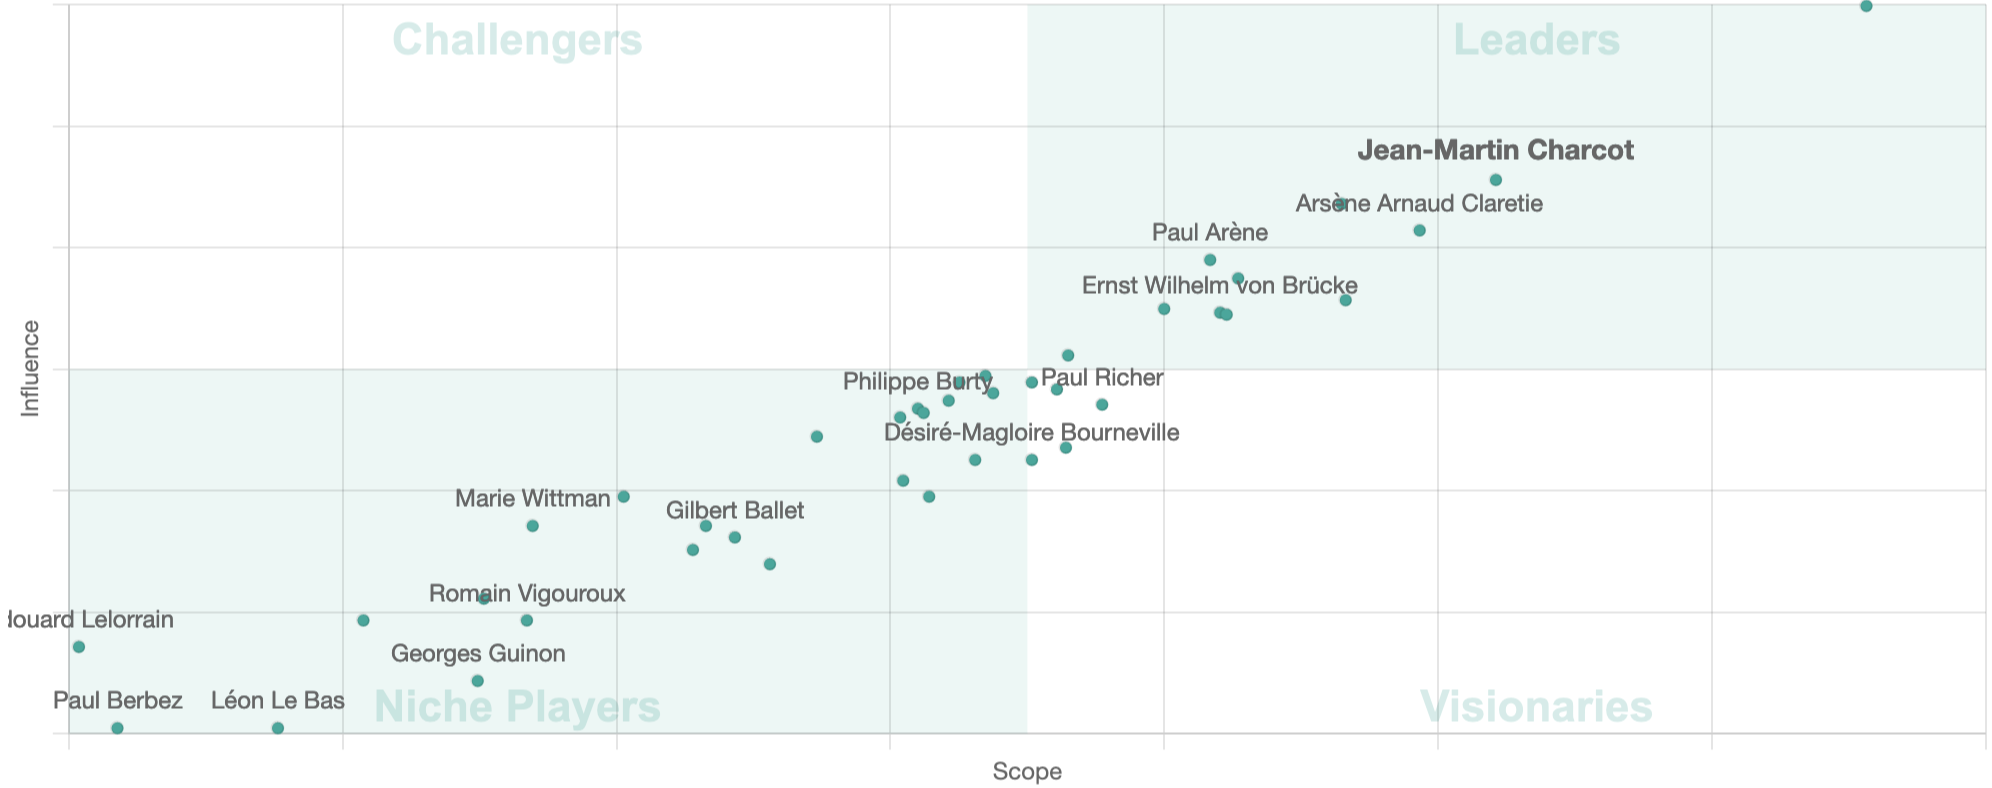
\includegraphics[width=1\textwidth]{img/analyse_quadrant.png}
    \caption[Positionnement de l'entité \texttt{Jean-Martin Charcot} au sein de son domaine et comparaison avec les entités les plus similaires à lui \textit{via} une analyse de quadrant de l'outil Rankingdom.]{Positionnement de l'entité \texttt{Jean-Martin Charcot} au sein de son domaine et comparaison avec les entités les plus similaires à lui \textit{via} une analyse de quadrant de l'outil Rankingdom\protect\footnotemark{.}}
    % Pour raison de visibilité, l'image originale a été agrandie, ce qui a entraîné le rapprochement des années sur l'axe de l'abscisse.
    \label{fig:analyse_quadrant}
\end{figure}

\footnotetext{\url{https://www.rankingdom.org/entity/Q20710?search=jean-martin+charcot}. Le domaine dans lequel Charcot figure est relativement large, y compris les figures du domaine médical (p. ex. Bourneville), mais aussi littéraire (Arsène Arnaud Claretie).}

\bigskip
L'impact de Charcot peut également être visualisé à l'aide de Rankingdom à travers le graphique qui apporte une dimension temporelle (figure \ref{fig:impact_temporel}). Il s'agit notamment de la cumulation temporelle de son impact, où l'on peut observer qu'il s'étend sur la période 1856--1994. 

\begin{figure}[hb]
    \centering
    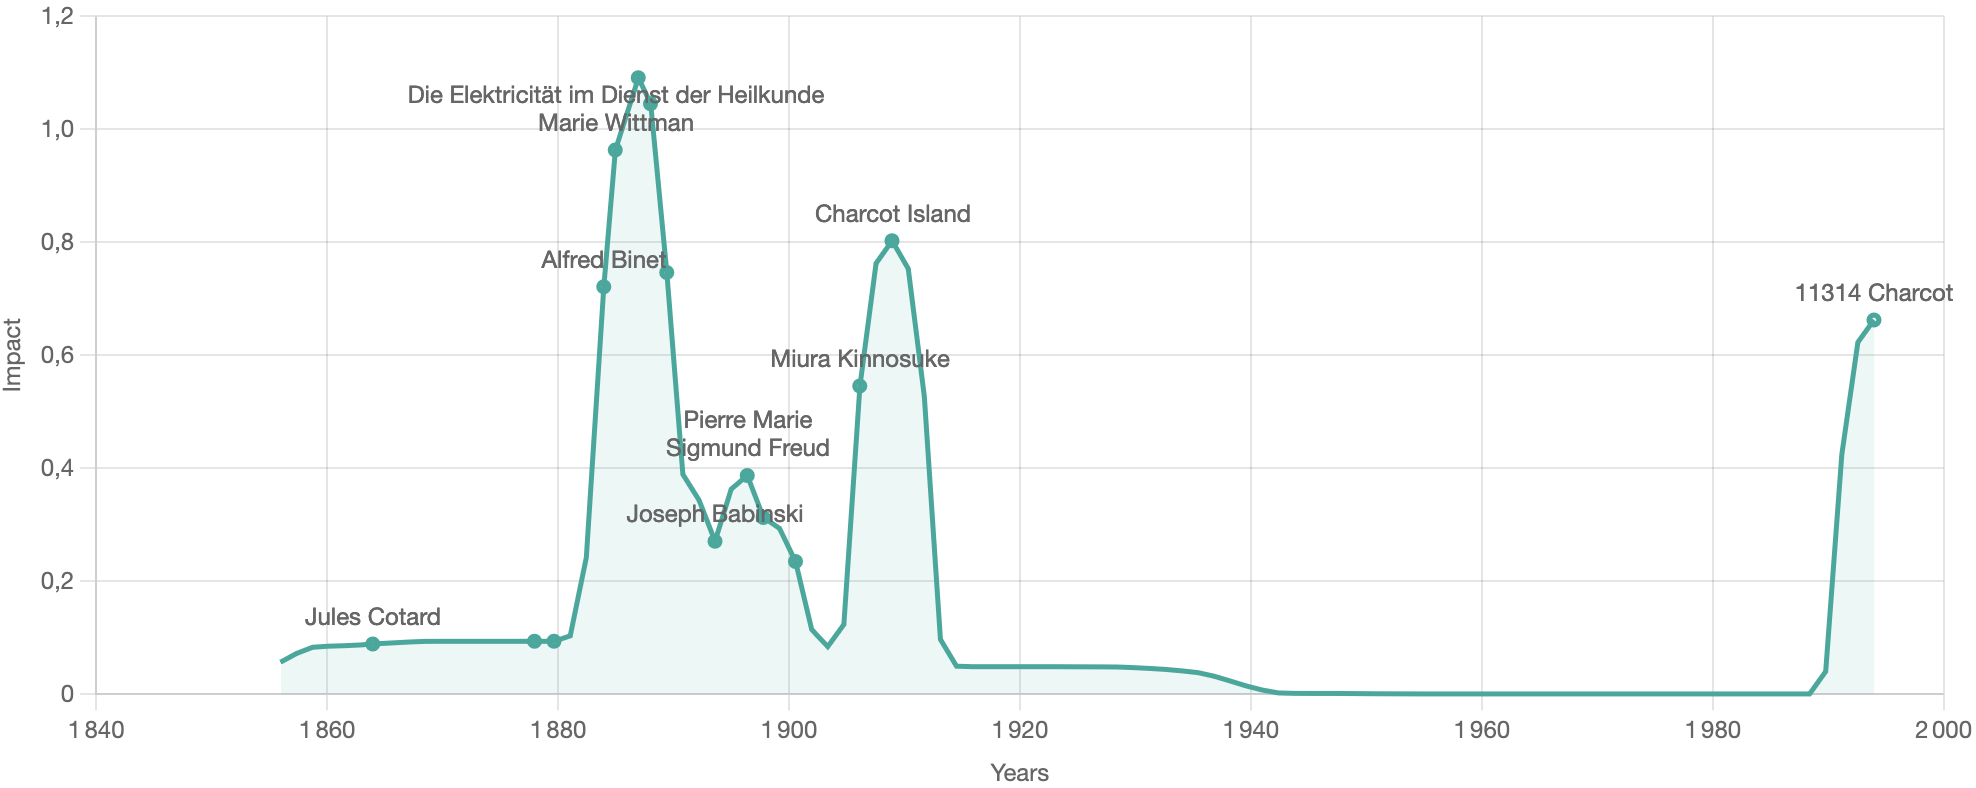
\includegraphics[width=1\textwidth]{img/impact_temporel.png}
    \caption[Analyse temporelle de l'impact de l'entité \texttt{Jean-Martin Charcot} à l'aide de l'outil Rankingdom.]{Analyse temporelle de l'impact de l'entité \texttt{Jean-Martin Charcot} à l'aide de l'outil Rankingdom\protect\footnotemark{.}}
    % Pour raison de visibilité, l'image originale a été agrandie, ce qui a entraîné le rapprochement des années sur l'axe de l'abscisse.
    \label{fig:impact_temporel}
\end{figure}

\footnotetext{\url{https://www.rankingdom.org/entity/Q20710?search=jean-martin+charcot}.}

Enfin, il est également possible de lister les entités impactées, comprenant les personnes (p. ex. Sigmund Freud), les notions médicales (SEP) ou bien les entités géographiques afférentes (Île Charcot).


%Les humanités numériques au service de l'analyse des circulations culturelles
%
%Comment définir une circulation du point de vue de l'analyse du texte ? de la linguistique computationnelle (TAL) ?
